

\tikzset{every picture/.style={line width=0.75pt}} %set default line width to 0.75pt        

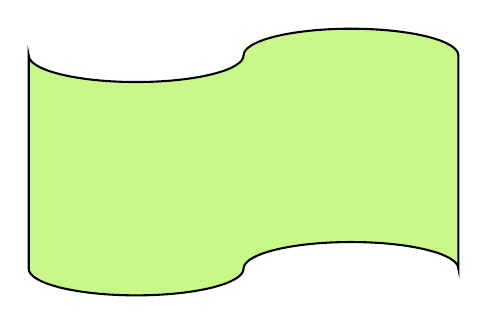
\begin{tikzpicture}[x=0.75pt,y=0.75pt,yscale=-1,xscale=1]
%uncomment if require: \path (0,300); %set diagram left start at 0, and has height of 300

%Flowchart: Punched Tape [id:dp25700721970086793] 
\draw  [fill={rgb, 255:red, 201; green, 248; blue, 137 }  ,fill opacity=1 ] (155,67.85) .. controls (155,74.94) and (178.17,80.69) .. (206.75,80.69) .. controls (235.33,80.69) and (258.5,74.94) .. (258.5,67.85) .. controls (258.5,60.75) and (281.67,55) .. (310.25,55) .. controls (338.83,55) and (362,60.75) .. (362,67.85) -- (362,170.62) .. controls (362,163.52) and (338.83,157.77) .. (310.25,157.77) .. controls (281.67,157.77) and (258.5,163.52) .. (258.5,170.62) .. controls (258.5,177.72) and (235.33,183.47) .. (206.75,183.47) .. controls (178.17,183.47) and (155,177.72) .. (155,170.62) -- cycle ;




\end{tikzpicture}
